\documentclass{article}
\usepackage[utf8]{inputenc}
\usepackage[margin=4em]{geometry}

\usepackage{xcolor}
\usepackage{amsmath,amssymb}
\usepackage{cancel}
\usepackage{pifont}
\usepackage{pgfplots}
\pgfplotsset{compat = newest}

\def\chk{\ding{51}}
\def\xhk{\ding{55}}
\def\em{\hspace{1em}}
\newcommand{\cell}[1]{\hspace{-.5em}&#1&\hspace{-.5em}}
\def\eqa{\cell{=}}
\def\>{\rightarrow}
\newcommand{\subtag}[1]{\tag{\theparentequation#1}}

\title{Chapter 1 Notes}
\author{Cole Gannon}
\date{}

\begin{document}
\maketitle

\section{Linear Equations (in General)}

Each variable within the equation such as $x$, $y$, or $z$, for example, must
have either exponent $1$ or $0$.

\begin{itemize}
   \item \chk\ $2x+1=7$
   \item \xhk\ $x^{\textcolor{red}{2}}=2y$
   \item \xhk\ $\textcolor{red}{\sin(x)}=2x$
   \item \xhk\ $\textcolor{red}{\sqrt{x}}=3x+1$
\end{itemize}

\begin{center}
   \textbf{Def}: Linear Equation\\
   $a_1v_1+a_2v_2+a_3v_3+\cdots+a_nv_n=b$\\
   \hspace{-5em}\textit{where:}\\
   \vspace{-2em}
   \begin{align*}
      \forall a&\in\mathbb{R}\\
      b&\in\mathbb{R}
   \end{align*}

   \textbf{Def}: System of Linear Equations / Linear System / L.S.\\
   A collection of one or more linear equations.\\
   (One linear equation only would be kinda silly,
   though it technically qualifies.)
\end{center}

\subsection{Solutions}

\subsubsection{A Solution}
\begin{center}
   \textbf{Def}: \textit{A} Solution of a Linear System\\
   Given a L.S. in $x_1, x_2, x_3 \cdots x_n$ or $\mathbb{R}^n$,
   \textit{A} solution is an n-tuple corresponding to each respective variable.
   $\left(S_1, S_2, S_3, \cdots, S_n\right)$,
\end{center}
Let's work an example:
\begin{flalign}
   \left\{
      \begin{matrix}
           x+2y\eqa5
         \\2x+y\eqa10
      \end{matrix}
   \right\}
   \tag{ex. A}
   \begin{array}{ll}
      x=5-2y
      \> 2[x=5-2y]+y=10
      \> \cancel{10}-2y+y=\cancel{10}
      \> \mathbf{y=0}
      \\
      x=5-2[y=0]
      \> \mathbf{x=5}
      \\
      $The solution is\ $ (x,y) = (5,0)
   \end{array}
   &&
\end{flalign}

\subsubsection{Solution Sets}
\begin{center}
   \textbf{Def}: The Solution Set of a Linear System\\
   The set of all possible solutions for a given L.S.
\end{center}
In the example in 1.1.1, there was only one possible solution: (5,0).
Therefore, the solution set of ex. A is \{(5, 0)\}.

\begin{flalign*}
   &\left\{x+2y=1\right\}
   \tag{ex. B}
   \\
   &\hspace{-3px} \Rightarrow\ \left\{(x,y)\ | \ x+2y=1\right\}
   \\
   & \textit{or}\ \left\{(x,\frac{1-x}{2})\ |\ \forall x \in \mathbb{R}\right\}
   \\
   & \textit{or}\ \left\{(1-2y,y)\ |\ \forall y \in \mathbb{R}\right\}
   &&
\end{flalign*}
\\

The notation you see above is the Set builder notation.\\
$\left\{x\ |\ \forall\ x \in \mathbb{Z} \text{, modulo}(x, 2) = 0 \right\}$
should be read as ``the set of all integers $x$ where $x$ mod two is zero.''.
This is the set of all even numbers.

\pagebreak

\subsubsection{The Existence and Uniqueness Questions}
So when we have a linear system, something we like to ask is
``Does a solution exist?''. If a solution exists,
``Does a unique solution exist?''. These are \textit{The Existence and Uniqueness Questions}.
There are three solution states for any given linear system.

\begin{itemize}
   \item No Solution $\cancel{\exists}$
   \item Unique Solution $\exists!$
   \item Infinitely Many Solutions $\exists\infty$-many
\end{itemize}

\begin{tabular}{c c c}
   $\left\{
      \begin{matrix}
         \textcolor{magenta}{x+2y}\cell{\textcolor{magenta}{=}}\textcolor{magenta}{1}\\
         \textcolor{orange}{2x-4y}\cell{\textcolor{orange}{=}}\textcolor{orange}{0}
      \end{matrix}
   \right\}
   \cancel{\exists}
   $
   sln.
   &
   $\left\{
      \begin{matrix}
         \textcolor{magenta}{x+2y}\cell{\textcolor{magenta}{=}}\textcolor{magenta}{1}\\
         \textcolor{olive}{x-y}\cell{\textcolor{olive}{=}}\textcolor{olive}{0}
      \end{matrix}
   \right\}
   \exists!
   $
   sln.
   &
   $\left\{
      \begin{matrix}
         \textcolor{magenta}{x+2y}\cell{\textcolor{magenta}{=}}\textcolor{magenta}{1}\\
         \textcolor{teal}{2x+4y}\cell{\textcolor{teal}{=}}\textcolor{teal}{2}
      \end{matrix}
   \right\}
   \exists\infty
   $
   sln.
   \\
   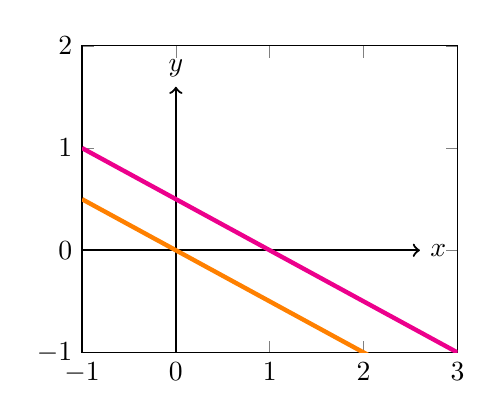
\begin{tikzpicture}
      \begin{axis}[xmin=-1,xmax=3,ymin=-1,ymax=2,width=180px]
         \draw[->,thick](-1,0)--(2.6,0)node[right]{$x$};
         \draw[->,thick](0,-1)--(0,1.6)node[above]{$y$};
         \addplot[domain=-1:3,samples=40,smooth,ultra thick,magenta]{(1-x)/2};
         \addplot[domain=-1:3,samples=40,smooth,ultra thick,orange]{-x/2};
     \end{axis}
   \end{tikzpicture}
   &
   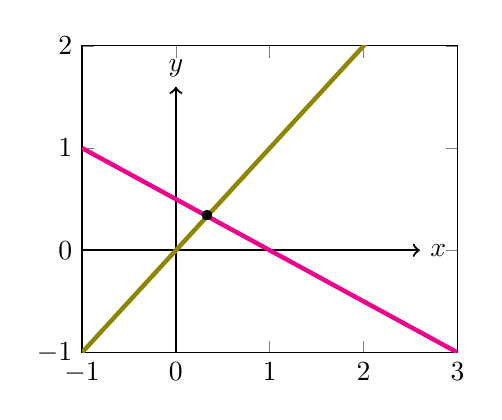
\begin{tikzpicture}
      \begin{axis}[xmin=-1,xmax=3,ymin=-1,ymax=2,width=180px]
         \draw[->,thick](-1,0)--(2.6,0)node[right]{$x$};
         \draw[->,thick](0,-1)--(0,1.6)node[above]{$y$};
         \addplot[domain=-1:3,samples=40,smooth,ultra thick,magenta]{(1-x)/2};
         \addplot[domain=-1:3,samples=40,smooth,ultra thick,olive]{x};
         \draw (1/3,1/3)node{\textbullet};
     \end{axis}
   \end{tikzpicture}
   &
   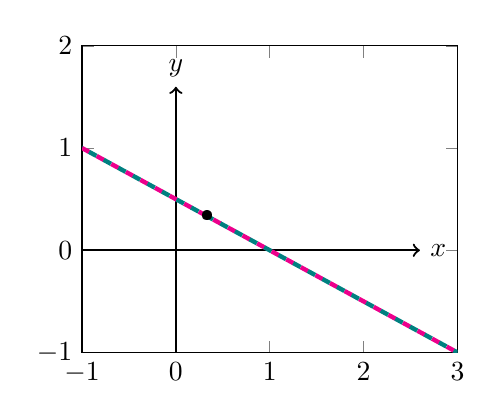
\begin{tikzpicture}
      \begin{axis}[xmin=-1,xmax=3,ymin=-1,ymax=2,width=180px]
         \draw[->,thick](-1,0)--(2.6,0)node[right]{$x$};
         \draw[->,thick](0,-1)--(0,1.6)node[above]{$y$};
         \addplot[domain=-1:3,samples=20,dashed,ultra thick,magenta]{(1-x)/2};
         \addplot[domain=-1.08:3.08,samples=20,dashed,ultra thick,teal]{(1-x)/2};
         \draw (1/3,1/3)node{\textbullet};
     \end{axis}
   \end{tikzpicture}
\end{tabular}

\subsection{Determination}
\begin{flalign*}
   \left\{
      \begin{matrix}
           2x+y\eqa3-x
         \\x-y \eqa5
         \\x+2y\eqa1
      \end{matrix}
   \right\}
   &
   \hspace{2em}
   \begin{array}{ll}
      \text{Linear System of\ } x \text{\ and\ } y\text{.}\\
      % So when in a math environment, turns out that the dollar sign undoes it.
      % Both the above \text and below $ are valid ways to do this.
      % :scrumge:
      $Overdetermined; three equations when there are only two variables.$
   \end{array}
   \\
   \\
   \left\{
      \vspace{.5em}
      \begin{matrix}
           x-y+z  \eqa 1
         \\2x+y-z \eqa 3
      \end{matrix}
      \vspace{.5em}
   \right\}
   &
   \hspace{2em}
   \begin{array}{ll}
        $Linear System of\ $ x $,\ $ y $, and\ $ z$.$
      \\$Underdetermined; two equations when there are three variables.$
   \end{array}
   &&
\end{flalign*}

Keep in mind that determination alone is not a sufficient indicator of the
existence of a solution. We'll touch on this more in

\end{document}
